
U odred1enim situacijama mozhe doc1i do promene zahteva (bolest vozacha, neprijavljen kvar vozila i sl.). Tada je neophodno da logistichari izmene informacije o zahtevu.

\begin{enumerate}
    \item \textbf{Kratak opis:} Logistichar menja informacije o zahtevu. Moguc1e je menjanje rute, vozacha, vozila, procenjene cene ili vremena izvrshenja transporta. 
    
    \item \textbf{Uchesnici:} Logistichar, Vozach, Magacioner.
    \item \textbf{Preduslovi:} Sistem je u funkciji. Zahtev je aktivan.
    \item \textbf{Postuslovi:} Zahtev za transport je izmenjen. Informacije o izmeni zahteva su zabelezhene. Magacioner i Vozach je primio informaciju da je doshlo do izmene u zahtevu.
    \item \textbf{Osnovni tok:}
        \begin{enumerate}
            \item[5.1.] Logishtichar pristupa sistemu. 
            \item[5.2.] Na osnovu ID zahteva pristupa informacijama o zahtevu.
            
            \item[5.3.] Logistichar menja zheljene informacije. 
            \item[5.4.] Logistichar potvrd1uje izmene klikom na dugme.
            
            \item[5.5.] Sistem chuva informacije o izmeni zahteva.
            \item[5.6.] Izveshtaj sa izmenama se shalje Magacioneru.
            \item[5.7.] Izveshtaj sa izmenama se shalje svim Vozachima.
            
        \end{enumerate}
    \item \textbf{Alternativni tokovi:}
            \begin{enumerate}
                \item [A1.] \textbf{Greshka prilikom unosa ID poshiljke: }
                Ukoliko u koraku 5.2. Logistichar unese pogreshan ID, sistem ga obaveshtava da je doshlo do greshke. 
                Nakon shto se ispravi greshku, proces se nastavlja u koraku 5.2.
            \end{enumerate}
        
    \item \textbf{Podtokovi:} /
    \item \textbf{Specijalni zahtevi:} /
    \item \textbf{Dodatne informacije:} Izveshtaji sadrzhe informacije kao u zahtevu Obrada zahteva.
    
\end{enumerate}



\begin{figure}[H]
    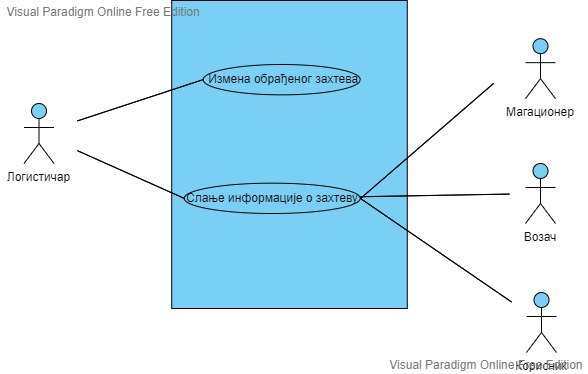
\includegraphics[scale=0.5]{Slike/UML/SUizmenaZahteva.jpg}
    \centering
    \caption{Sluchaj upotrebe: Izmena zahteva za transport}
    \label{dsizmena}
\end{figure}    

\newpage


